\documentclass[conference]{IEEEtran}
\usepackage[T1]{fontenc}
\usepackage{amsmath,amssymb}
\usepackage{booktabs}
\usepackage{xcolor}
\usepackage{tikz}
\usetikzlibrary{arrows.meta,positioning,calc}
\usepackage{listings}
\usepackage{pgfplots}
\pgfplotsset{compat=1.18}
\usepackage{xurl}

\newcommand{\sys}{\textsc{DeltaProof}}
\newcommand{\repo}{\url{https://github.com/nithinnnv/deltaproof}}
\lstset{basicstyle=\ttfamily\scriptsize, columns=fullflexible, keepspaces=true, frame=single, framesep=2pt,
  xleftmargin=3pt, xrightmargin=3pt, aboveskip=4pt, belowskip=2pt, breaklines=true}

\begin{document}

\title{\sys{}: Finding the Exact Rows That Differ After a Heterogeneous Database Migration}

\author{\IEEEauthorblockN{Nithin Narla}
\IEEEauthorblockA{Independent Researcher\\
nithin.nnv@gmail.com}}

\maketitle

\begin{abstract}
When a system is re-engineered onto a different database, for example from PostgreSQL to Cassandra, its owners must show that the migrated data matches the original before they cut over. Existing tools compare row counts and aggregates, which miss value errors, or compare every row, which costs a full read of both databases and fails when the two stores order and encode records differently. \sys{} is an open-source command-line tool and Python library that reports the exact keys that are missing, extra or different between two databases. A canonical encoder makes logically equal records hash identically across stores, and each store is summarized by a small sketch built from invertible Bloom lookup tables, whose comparison costs bytes proportional to the number of differences rather than the size of the tables. Sketches can be built next to each store and compared anywhere, and they can be maintained from a change stream while the migration is live. On TPC-H \texttt{lineitem} loaded into PostgreSQL and Cassandra, \sys{} found every injected fault with no false positives while exchanging 260\,KB for 6 million rows; a checksum of the drivers' raw values flagged every row. Tool: \repo{}.
\end{abstract}

\begin{IEEEkeywords}
data migration, reengineering, data validation, set reconciliation, NoSQL
\end{IEEEkeywords}

\section{Introduction}
Moving a system's data to a different database is a common reengineering step: a relational store is replaced by a wide-column store to scale writes, or a legacy schema is rebuilt in a new one. The migration is complete only when the target provably holds the same data as the source. In practice teams check row counts or column sums, which pass when a value is rounded, a timestamp is shifted or a lost row is offset by a duplicate, or they read and compare every row, which loads both production databases and grows with table size. Key-range checksum tools such as data-diff~\cite{datadiff} and pt-table-checksum~\cite{ptchecksum} reduce transfer but require both stores to scan in the same key order, which hash-partitioned stores such as Cassandra~\cite{lakshman2010} do not provide.

Two problems make heterogeneous verification hard. First, the same logical record has different physical forms: PostgreSQL returns \texttt{CHAR(25)} values padded with spaces and Cassandra returns them trimmed; one driver returns a \texttt{date}, the other its own date type; decimals, time zones and timestamp precision differ. A checksum over raw values reports nearly every row as different. Second, the useful answer is the list of differing keys, which is usually tiny compared with the tables.

\sys{} addresses both. It treats verification as set reconciliation~\cite{eppstein2011}: each store becomes a set of (key, value digest) elements under a canonical encoding, and the tool computes the symmetric difference of the two sets. It contributes:
\begin{itemize}
\item a command-line tool that, given a short table specification and two connection URLs, prints every missing, extra and mismatched key (Section~\ref{sec:use});
\item a canonical record encoder for relational and wide-column stores (Section~\ref{sec:arch});
\item a sketch format, built from invertible Bloom lookup tables (IBLTs)~\cite{goodrich2011}, that can be produced next to each store, shipped as a file, and compared in bytes proportional to the number of differences;
\item an evaluation on PostgreSQL and Cassandra with injected faults (Section~\ref{sec:eval}).
\end{itemize}

\section{Using \sys{}}\label{sec:use}
\subsection{Describing the tables}
The user writes a specification that names each table's primary key and its non-key columns with a logical type. The type, not the stores' physical types, decides when two values are equal: \texttt{d2} is an exact decimal at scale 2, \texttt{c} a fixed-width string whose padding is ignored, \texttt{dt} a calendar date, \texttt{ts} a UTC timestamp at milliseconds, and a trailing \texttt{?} allows nulls. Listing~\ref{lst:spec} shows the specification used for TPC-H \texttt{lineitem}. One specification can list many tables; they are compared together.

\begin{lstlisting}[caption={Table specification (\texttt{lineitem.toml})}, label={lst:spec}]
[[table]]
name = "lineitem"
key = ["l_orderkey", "l_linenumber"]
columns = """l_partkey:i l_suppkey:i l_quantity:d2
  l_extendedprice:d2 l_discount:d2 l_tax:d2
  l_returnflag:c l_linestatus:c l_shipdate:dt
  l_commitdate:dt l_receiptdate:dt l_shipinstruct:c
  l_shipmode:c l_comment:t"""
\end{lstlisting}

\subsection{Running a comparison}
The simplest use compares two live databases in one command (Listing~\ref{lst:run}, run with \texttt{--limit 1}). When the stores sit in different networks, \texttt{deltaproof sketch} runs next to each store and writes a sketch file, and \texttt{deltaproof diff} compares the two files anywhere. A file holding every size of sketch is about 20 bytes per row, little less than the rows' digests themselves; with \texttt{--max-differences 1000} it holds only the sizes needed for up to 1{,}000 differences, 232\,KB for 600{,}000 rows. If more differences turn up, \texttt{diff} falls back to an exact comparison of the stores named by \texttt{--source} and \texttt{--target}. The exit status is 0 when the stores match and 1 otherwise, so the command can gate a cutover script or a CI job, and \texttt{--json} prints a machine-readable report.

\begin{lstlisting}[caption={Comparing PostgreSQL with Cassandra}, label={lst:run}]
$ deltaproof verify --spec lineitem.toml \
    --source postgresql://user:pw@pg:5432/tpch \
    --target cassandra://cass:9042/tpch
120 differing keys
  missing_in_target: 20
    table=lineitem l_orderkey=11655 l_linenumber=3
    ... 19 more (use --limit -1 or --json)
  extra_in_target: 40
    table=lineitem l_orderkey=18277 l_linenumber=2
    ... 39 more (use --limit -1 or --json)
  value_mismatch: 60
    table=lineitem l_orderkey=11683 l_linenumber=5
    ... 59 more (use --limit -1 or --json)
compared 260,496 bytes of sketch in 2 round trips;
rescanned 0 rows
\end{lstlisting}

\subsection{Verifying while the migration is live}
The library exposes the same sketches as objects that accept inserts, updates and deletes. Fed from a change-data-capture stream on the source and from the replicator's writes on the target, they stay equal to sketches rebuilt from scratch, so a migration can be checked every few seconds without rescanning. A watermark and a version check on the target separate writes still in flight from real divergence; this mode, its correctness argument and its evaluation under a TPC-C workload are the subject of a companion paper, and the scripts that run it are in the repository.

\section{Architecture}\label{sec:arch}
\begin{figure}[t]
\centering
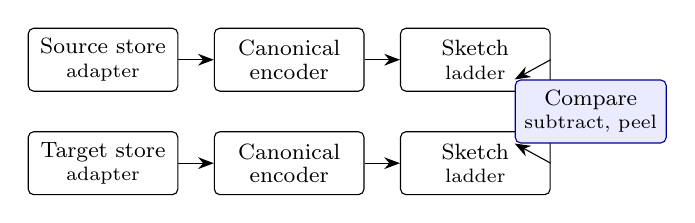
\begin{tikzpicture}[font=\footnotesize, box/.style={draw, rounded corners=2pt, minimum width=1.9cm, minimum height=0.8cm, align=center}, >={Stealth[length=2mm]}]
\node[box] (pg) {Source store\\[-1pt]\scriptsize adapter};
\node[box, below=0.5cm of pg] (cs) {Target store\\[-1pt]\scriptsize adapter};
\node[box, right=0.45cm of pg] (ce) {Canonical\\[-1pt]encoder};
\node[box, right=0.45cm of cs] (ct) {Canonical\\[-1pt]encoder};
\node[box, right=0.45cm of ce] (ss) {Sketch\\[-1pt]\scriptsize ladder};
\node[box, right=0.45cm of ct] (ts) {Sketch\\[-1pt]\scriptsize ladder};
\node[box, right=0.5cm of $(ss)!0.5!(ts)$, fill=blue!8, draw=blue!60!black] (co) {Compare\\[-1pt]\scriptsize subtract, peel};
\draw[->] (pg) -- (ce); \draw[->] (ce) -- (ss);
\draw[->] (cs) -- (ct); \draw[->] (ct) -- (ts);
\draw[->] (ss.east) -- (co.north west);
\draw[->] (ts.east) -- (co.south west);
\end{tikzpicture}
\caption{Pipeline. Each side can run next to its store; only sketches travel.}
\label{fig:arch}
\end{figure}

Fig.~\ref{fig:arch} shows the pipeline. The library and command line are about 1{,}200 lines of Python with NumPy; baselines and benchmarks are separate.

\emph{Adapters} read rows through each database's driver (psycopg~3 for PostgreSQL, the DataStax driver for Cassandra) and convert driver values to logical Python values; a new store needs only an adapter that yields rows as dictionaries.

\emph{The canonical encoder} turns a row into an element: a 128-bit key and a 64-bit digest of the values. Decimals become integers at the declared scale, so \texttt{10.5} and \texttt{10.50} agree; timestamps become UTC at the declared unit, so a store that keeps microseconds agrees with one that keeps milliseconds; text is Unicode NFC, hashed with BLAKE2b; fixed-width strings drop their padding; floats are compared by their IEEE-754 bits; and nulls carry their own tag, so null, the empty string and zero differ. Composite keys of up to four integer columns are packed with an 8-bit table tag, which lets one sketch cover many tables and lets a reported key be turned back into table and column values.

Table~\ref{tab:forms} lists differences between the two drivers' forms of the same logical value that the encoder absorbs. On \texttt{lineitem}, the first two alone made a raw-value checksum flag every row.

\begin{table}[t]
\caption{Same value, different driver forms, one canonical form}
\label{tab:forms}
\centering\footnotesize
\setlength{\tabcolsep}{2.5pt}
\begin{tabular}{@{}llll@{}}
\toprule
Type & PostgreSQL & Cassandra & Canonical\\
\midrule
\texttt{CHAR(10)} & \texttt{'MAIL\ \ \ \ \ \ '} & \texttt{'MAIL'} & trimmed, NFC\\
date & \texttt{date} & \texttt{util.Date} & days since 1970\\
timestamp & \textmu s & naive UTC, ms & UTC, set unit\\
decimal & column scale & value's scale & scaled integer\\
\bottomrule
\end{tabular}
\end{table}

\emph{Sketches.} An IBLT is an array of cells; each element is added to three cells, and each cell keeps a count and XOR sums of keys, digests and a checksum~\cite{goodrich2011}. Subtracting the target's IBLT from the source's cancels every common element, and \emph{peeling} cells that hold a single element recovers the difference. The difference must fit the IBLT, but its size is unknown in advance, so each store keeps a \emph{ladder} of IBLTs at capacities $64\cdot8^i$ up to one eighth of the row count, split by key hash into partitions of about 256 differences each, plus a 32-level strata estimator~\cite{eppstein2011}. The comparison reads the estimator first, then the smallest level with 25\% headroom over the estimate. A partition that fails to peel is compared row by row, so an undersized estimate costs time, never correctness. The ladder adds about 17 bytes per row.

\emph{Engineering choices.} Partitioning by key hash rather than key range makes the result independent of each store's scan order. Building every ladder level at once costs little because an update touches three cells per level, and it lets one comparison pick the right size after seeing the estimate. Sketch files of two stores with different row counts remain comparable, because a smaller ladder is a prefix of a larger one. The vectorized NumPy path and the scalar path used while peeling are bit-identical, which the tests check.

\section{Evaluation}\label{sec:eval}
We ran PostgreSQL~16.4 and Cassandra~4.1.6 as single nodes in Docker on one Apple M1 Pro laptop (10 cores, 16\,GB), with Python~3.13. Faults were injected with SQL and CQL statements, and the ground truth was the exact difference of full scans of both stores.

\emph{Does it find the differences?} On a 200{,}000-row synthetic ledger with 120 faults of six classes, and on TPC-H \texttt{lineitem} at scale factors 0.1 and 1 with 120 faults (lost writes, decimal precision, shifted dates, corrupted text, lost deletes, phantom rows), \sys{} reported exactly the injected keys, with no false positives (Table~\ref{tab:e2e}). A digest of the drivers' raw values, without canonical encoding, flagged 99.9\% of ledger rows and every \texttt{lineitem} row: the stores format timestamps, padded strings and dates differently. TPC-H data was generated with \texttt{dbgen}; these are not TPC-H benchmark results. At SF~0.1 we also ran the \texttt{deltaproof} command itself in all three ways (one command; files with every size; files limited to 1{,}000 differences), and each printed the same 120 keys.

\begin{table}[t]
\caption{End-to-end runs, PostgreSQL vs.\ Cassandra}
\label{tab:e2e}
\centering\footnotesize
\setlength{\tabcolsep}{3pt}
\begin{tabular}{@{}lrrr@{}}
\toprule
& Ledger & \multicolumn{2}{c}{TPC-H \texttt{lineitem}}\\
\cmidrule(l){3-4}
& & SF 0.1 & SF 1\\
\midrule
Rows (source) & 200{,}000 & 600{,}552 & 6{,}001{,}215\\
Injected faults & 120 & 120 & 120\\
Found / false positives & 120 / 0 & 120 / 0 & 120 / 0\\
Sketch bytes compared & 260\,KB & 260\,KB & 260\,KB\\
Round trips & 2 & 2 & 2\\
Raw-value digest flags & 99.9\% & 100\% & 100\%\\
\bottomrule
\end{tabular}
\end{table}

\emph{What does it cost?} Comparing sketches took 12\,ms for the ledger and 0.16\,s for six million rows. The cost of a comparison follows the number of differences (Fig.~\ref{fig:bytes}): in a controlled in-process experiment with $10^7$ ledger rows and about 1{,}100 differences, \sys{} exchanged 0.78\,MB, while a Merkle tree exchanged 32\,MB, range-checksum bisection 280\,MB and a full comparison 480\,MB, each reporting the same keys.

\begin{figure}[t]
\centering
\begin{tikzpicture}
\begin{axis}[width=\columnwidth, height=4.6cm, xmode=log, ymode=log, xlabel={Differing keys}, ylabel={MB exchanged},
  legend style={font=\scriptsize, at={(0.5,-0.32)}, anchor=north, legend columns=4}, tick label style={font=\scriptsize}, label style={font=\footnotesize},
  ymin=0.1, ymax=1500, grid=major, grid style={gray!20}]
\addplot[blue!70!black, very thick, mark=*] table[x=d, y=deltaproof_mb] {../data/rq2_n10000000.dat};
\addplot[gray, mark=square*] table[x=d, y=merkle_mb] {../data/rq2_n10000000.dat};
\addplot[gray!70, mark=triangle*] table[x=d, y=bisection_mb] {../data/rq2_n10000000.dat};
\addplot[gray!50, mark=diamond*, dashed] table[x=d, y=full_scan_mb] {../data/rq2_n10000000.dat};
\legend{\sys{}, Merkle tree, Bisection, Full}
\end{axis}
\end{tikzpicture}
\caption{Bytes exchanged to find the differences among $10^7$ rows (log--log).}
\label{fig:bytes}
\end{figure} Building a sketch requires one scan of each store, the same as a full comparison; the savings are in transfer and in later checks, since a sketch maintained from a change stream needs no further scans. In Python, scanning, encoding and sketching \texttt{lineitem} took 18\,s on PostgreSQL and 28\,s on Cassandra at SF~0.1, and 243\,s and 495\,s at SF~1; this dominates the run time and is the first target for optimization.

\emph{Live mode.} Under a TPC-C workload replicated from PostgreSQL to Cassandra with injected drops and corruptions, sketches maintained from the change stream equalled full-scan rebuilds in every run, and checks every 10\,s reported no false differences; the companion paper reports this experiment in full.

\section{Related Tools}
\emph{Row counts and aggregates}, as offered by several migration services, are cheap but miss value faults. AWS DMS data validation~\cite{awsdms} compares rows between a migration task's source and target. Google's Data Validation Tool~\cite{dvt} compares counts, aggregates and row hashes across many databases, though not Cassandra. data-diff~\cite{datadiff} and pt-table-checksum~\cite{ptchecksum} checksum key ranges and narrow down mismatches, which needs both sides to scan in key order. Cassandra repairs replicas with Merkle trees~\cite{lakshman2010}, within one database and one encoding. \sys{} differs in comparing stores with different encodings and orders, in reporting exact keys from a transfer proportional to the number of differences, and in sketches that can be maintained from a change stream. IBLTs and strata estimators come from network set reconciliation~\cite{goodrich2011,eppstein2011}; PinSketch~\cite{minisketch} sends fewer bytes at a higher computational cost, and the encoder and pipeline would work with it as well.

\section{Limitations}
Keys must be integer columns (up to four, each below $2^{30}$) or UUIDs. Tables without a primary key cannot be compared key by key. The table specification must match the migration's intended mapping; if both sides were encoded wrongly in the same way, a mismatch would be hidden, so specifications need their own tests. Adapters exist for PostgreSQL and Cassandra only. Scans are row-by-row Python and therefore slow on large tables. A run with no differences still exchanges the 187\,KB estimator.

\section{Conclusion and Availability}
\sys{} turns migration verification into a short specification and one command, and returns the exact differing keys from two stores that encode and order data differently. The tool, tests, benchmark scripts, Docker setup and all result files are available under the Apache~2.0 license at \repo{}.

\section*{Acknowledgment}
The author used Claude (Anthropic) to write the tool's implementation, tests and benchmark scripts and to draft and edit the text of all sections of this paper, including the figure and tables. All results come from running that code. The author reviewed and takes responsibility for all content.

\begin{thebibliography}{9}
\bibitem{datadiff} data-diff, ``Technical explanation,'' project documentation. [Online]. Available: \url{https://data-diff.readthedocs.io/en/latest/technical-explanation.html}
\bibitem{ptchecksum} Percona, ``pt-table-checksum,'' Percona Toolkit documentation. [Online]. Available: \url{https://docs.percona.com/percona-toolkit/pt-table-checksum.html}
\bibitem{lakshman2010} A.~Lakshman and P.~Malik, ``Cassandra: A decentralized structured storage system,'' \emph{ACM SIGOPS Oper. Syst. Rev.}, vol.~44, no.~2, pp.~35--40, 2010.
\bibitem{goodrich2011} M.~T. Goodrich and M.~Mitzenmacher, ``Invertible Bloom lookup tables,'' in \emph{Proc. 49th Annu. Allerton Conf. Commun., Control, Comput.}, 2011, pp.~792--799.
\bibitem{eppstein2011} D.~Eppstein, M.~T. Goodrich, F.~Uyeda, and G.~Varghese, ``What's the difference? Efficient set reconciliation without prior context,'' in \emph{Proc. ACM SIGCOMM}, 2011, pp.~218--229.
\bibitem{awsdms} Amazon Web Services, ``AWS DMS data validation,'' AWS Database Migration Service User Guide. [Online]. Available: \url{https://docs.aws.amazon.com/dms/latest/userguide/CHAP_Validating.html}
\bibitem{dvt} Google Cloud, ``Data Validation Tool,'' GitHub repository. [Online]. Available: \url{https://github.com/GoogleCloudPlatform/professional-services-data-validator}
\bibitem{minisketch} P.~Wuille, G.~Maxwell, and G.~Naumenko, ``minisketch: An optimized library for BCH-based set reconciliation,'' GitHub repository. [Online]. Available: \url{https://github.com/bitcoin-core/minisketch}
\end{thebibliography}

\end{document}
